\documentclass[11pt]{exam}

\usepackage{amsmath}
\usepackage{graphicx}
\usepackage{geometry}
\usepackage{etoolbox}
\BeforeBeginEnvironment{choices}{\par\nopagebreak\minipage{\linewidth}}
\AfterEndEnvironment{choices}{\endminipage}
\geometry{
a4paper,
total={185mm,257mm},
left=10mm,
top=25mm,
bottom=10mm
}

\begin{document}
\setlength{\voffset}{-0.5in}
\setlength{\headsep}{5pt}

\fbox{\fbox{\parbox{8cm}{\centering
\vspace{2mm}
Testat - Versuch J - Ultraschall 
\vspace{2mm}
}}}
\hspace{2mm}
\makebox[0.25\textwidth]{Name:\enspace\hrulefill} \hspace{5mm}
\makebox[0.2\textwidth]{Datum:\enspace\hrulefill}
\vspace{4mm}

\begin{questions}

\question Wie hoch ist die Frequenz des in der Graphik dargestellten Signals? 

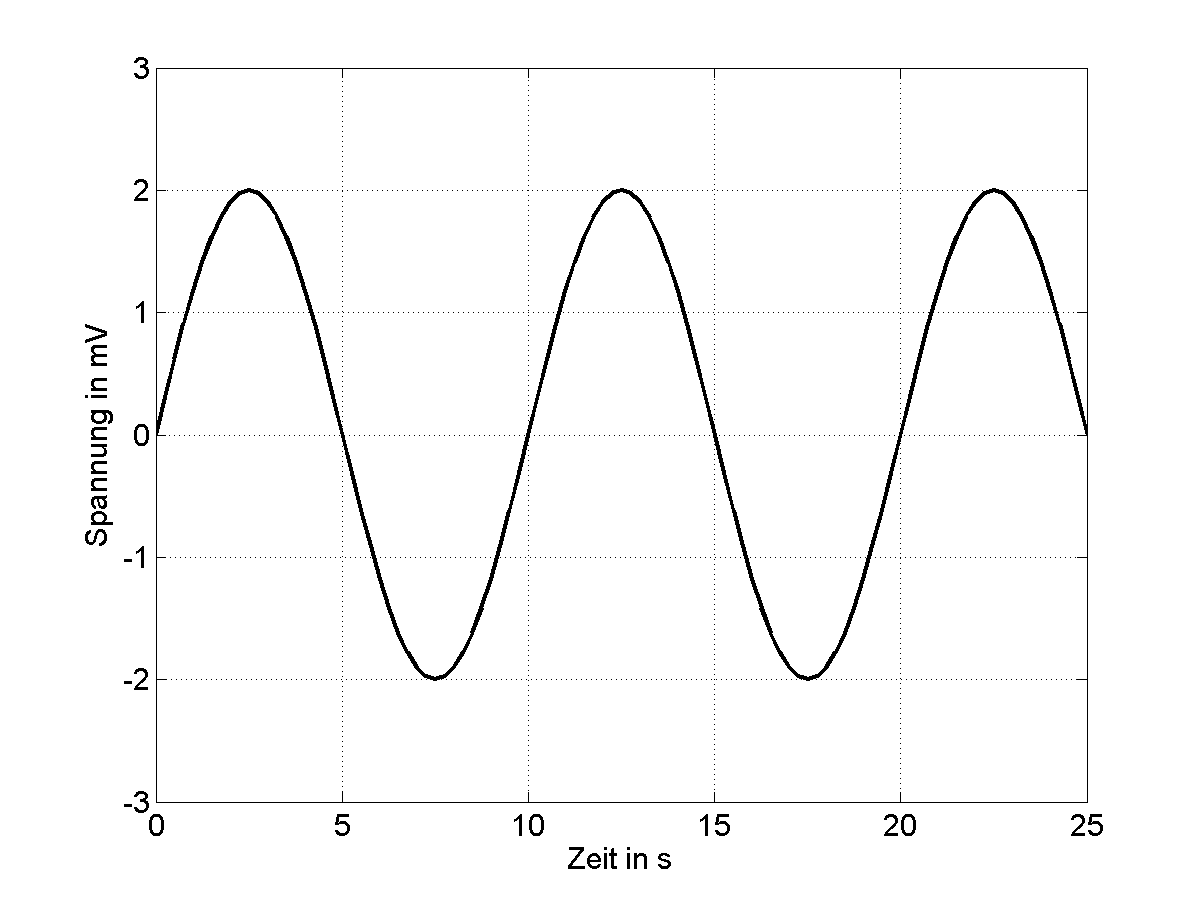
\includegraphics[width=0.4\textwidth]{images/SchallSinus1.png}

\begin{choices}
	\choice 0,2 Hz
	\choice 10 Hz
	\choice 10 s
	\choice 0,1 Hz (correct)
	\choice 5 s
\end{choices}

\vspace{3mm}\question Mit welcher Gleichung lässt sich der zurückgelegte Weg \( s \) eines Schallsignals beschreiben?( \( t \) Laufzeit des Signals, \( c \) Schallgeschwindigkeit )

\begin{choices}
	\choice \( s = c \cdot t^2 \)
	\choice \( s=c \cdot t \) (correct)
	\choice \( s= \frac{c}{t} \)
	\choice \( s=c^2 \cdot t \)
	\choice \( s= \frac{t}{c} \)
\end{choices}

\vspace{3mm}\question Welchen Weg \( s \) legt eine Schallwelle in einer Zeit  \( t= \mathrm{10~s} \) in Luft zurück?

\begin{choices}
	\choice 0,343 m
	\choice 34,3 m
	\choice 343 m
	\choice 3430 m (correct)
	\choice 3,43 m
\end{choices}

\vspace{3mm}\question Die Schallgeschwindigkeit...

\begin{choices}
	\choice ist im Vakuum größer als in Luft, da die Luftmoleküle die Schallübertragung dämpfen
	\choice hängt von der Amplitude der Schallwelle ab
	\choice ist bei zwei Schallwellen mit unterschiedlicher Frequenz gleich, wenn sie sich im gleichen Medium ausbreiten. (correct)
	\choice ist vom Übertragenden Medium unabhängig
	\choice Keine Antwort ist richtig.
\end{choices}

\vspace{3mm}\question Welche Aussagen zur Schallerzeugung und -ausbreitung sind zutreffend?	* Schallwellen können mit einem Piezo-Kristall erzeugt werden.	* Schallwellen können durch schwingende Membranen erzeugt werden.	* Die Schallgeschwindigkeit ist in Vakuum höher als in Luft, da die Schallwellen nicht durch Luftmoleküle gebremst werden.	* In Festkörpern ist die Schallgeschwindigkeit kleiner als in Luft, da die Moleküle nicht so schnell ausgelenkt werden können. 

\begin{choices}
	\choice Nur Ausage 1 und 3 sind richtig.
	\choice Nur Ausage 2 und 3 sind richtig.
	\choice Nur Ausage 2 und 4 sind richtig.
	\choice Nur Ausage 1 und 2 sind richtig. (correct)
	\choice Nur Ausage 3 und 4 sind richtig.
\end{choices}

\vspace{3mm}\end{questions}

\end{document}
